\documentclass[10pt,landscape]{article}
\usepackage[paperwidth=440mm,paperheight=300mm,margin=8mm]{geometry}
\usepackage[T1]{fontenc}
\usepackage[utf8]{inputenc}
\usepackage{tikz}
\usepackage{booktabs}
\usepackage{array}
\usepackage{xcolor}
\usepackage{amsmath}
\usepackage{hyperref}
\usetikzlibrary{arrows.meta,positioning,fit,calc}

\pagestyle{empty}
\setlength{\parindent}{0pt}
\renewcommand{\arraystretch}{1.12}

\definecolor{dataBlue}{RGB}{66,133,244}
\definecolor{condGreen}{RGB}{52,168,83}
\definecolor{edmOrange}{RGB}{239,108,0}
\definecolor{blockPurple}{RGB}{126,87,194}
\definecolor{lossRed}{RGB}{198,40,40}
\definecolor{grayBox}{RGB}{245,247,250}

\tikzset{
  tensor/.style={draw, rounded corners=2pt, very thick, fill=dataBlue!10, align=center, minimum height=9mm, font=\footnotesize},
  cond/.style={draw, rounded corners=2pt, very thick, fill=condGreen!10, align=center, minimum height=9mm, font=\footnotesize},
  op/.style={draw, rounded corners=2pt, very thick, fill=grayBox, align=center, minimum height=9mm, font=\footnotesize},
  edm/.style={draw, rounded corners=2pt, very thick, fill=edmOrange!12, align=center, minimum height=9mm, font=\footnotesize},
  unet/.style={draw, rounded corners=2pt, very thick, fill=edmOrange!10, align=left, minimum height=9mm, font=\scriptsize},
  block/.style={draw, rounded corners=2pt, very thick, fill=blockPurple!10, align=center, minimum height=9mm, font=\footnotesize},
  loss/.style={draw, rounded corners=2pt, very thick, fill=lossRed!8, align=center, minimum height=9mm, font=\footnotesize},
  arrow/.style={-{Latex[length=3mm]}, very thick},
  bus/.style={draw, rounded corners=2pt, thick, fill=condGreen!6, align=center, font=\scriptsize},
  note/.style={align=left, font=\footnotesize}
}

\newcommand{\shape}[1]{\texttt{[#1]}}
\newcommand{\cfg}{\texttt{dataset\_a\_256\_base48\_edm.yaml}}

\begin{document}

\begin{center}
{\Large EDM Conditional Diffusion Network for Ultrasonic Defect Map Inversion}\\[1mm]
{\normalsize Follows \cfg: image size 256, pic channels 8, x channels 7, frequencies 15, base channels 48.}\\
{\small All arrows are routed as horizontal/vertical orthogonal polylines. Tensor order: images \shape{B,C,H,W}; x-matrix \shape{B,C,F,TX,RX}; x tokens \shape{B,N,D}.}
\end{center}

\vspace{1mm}

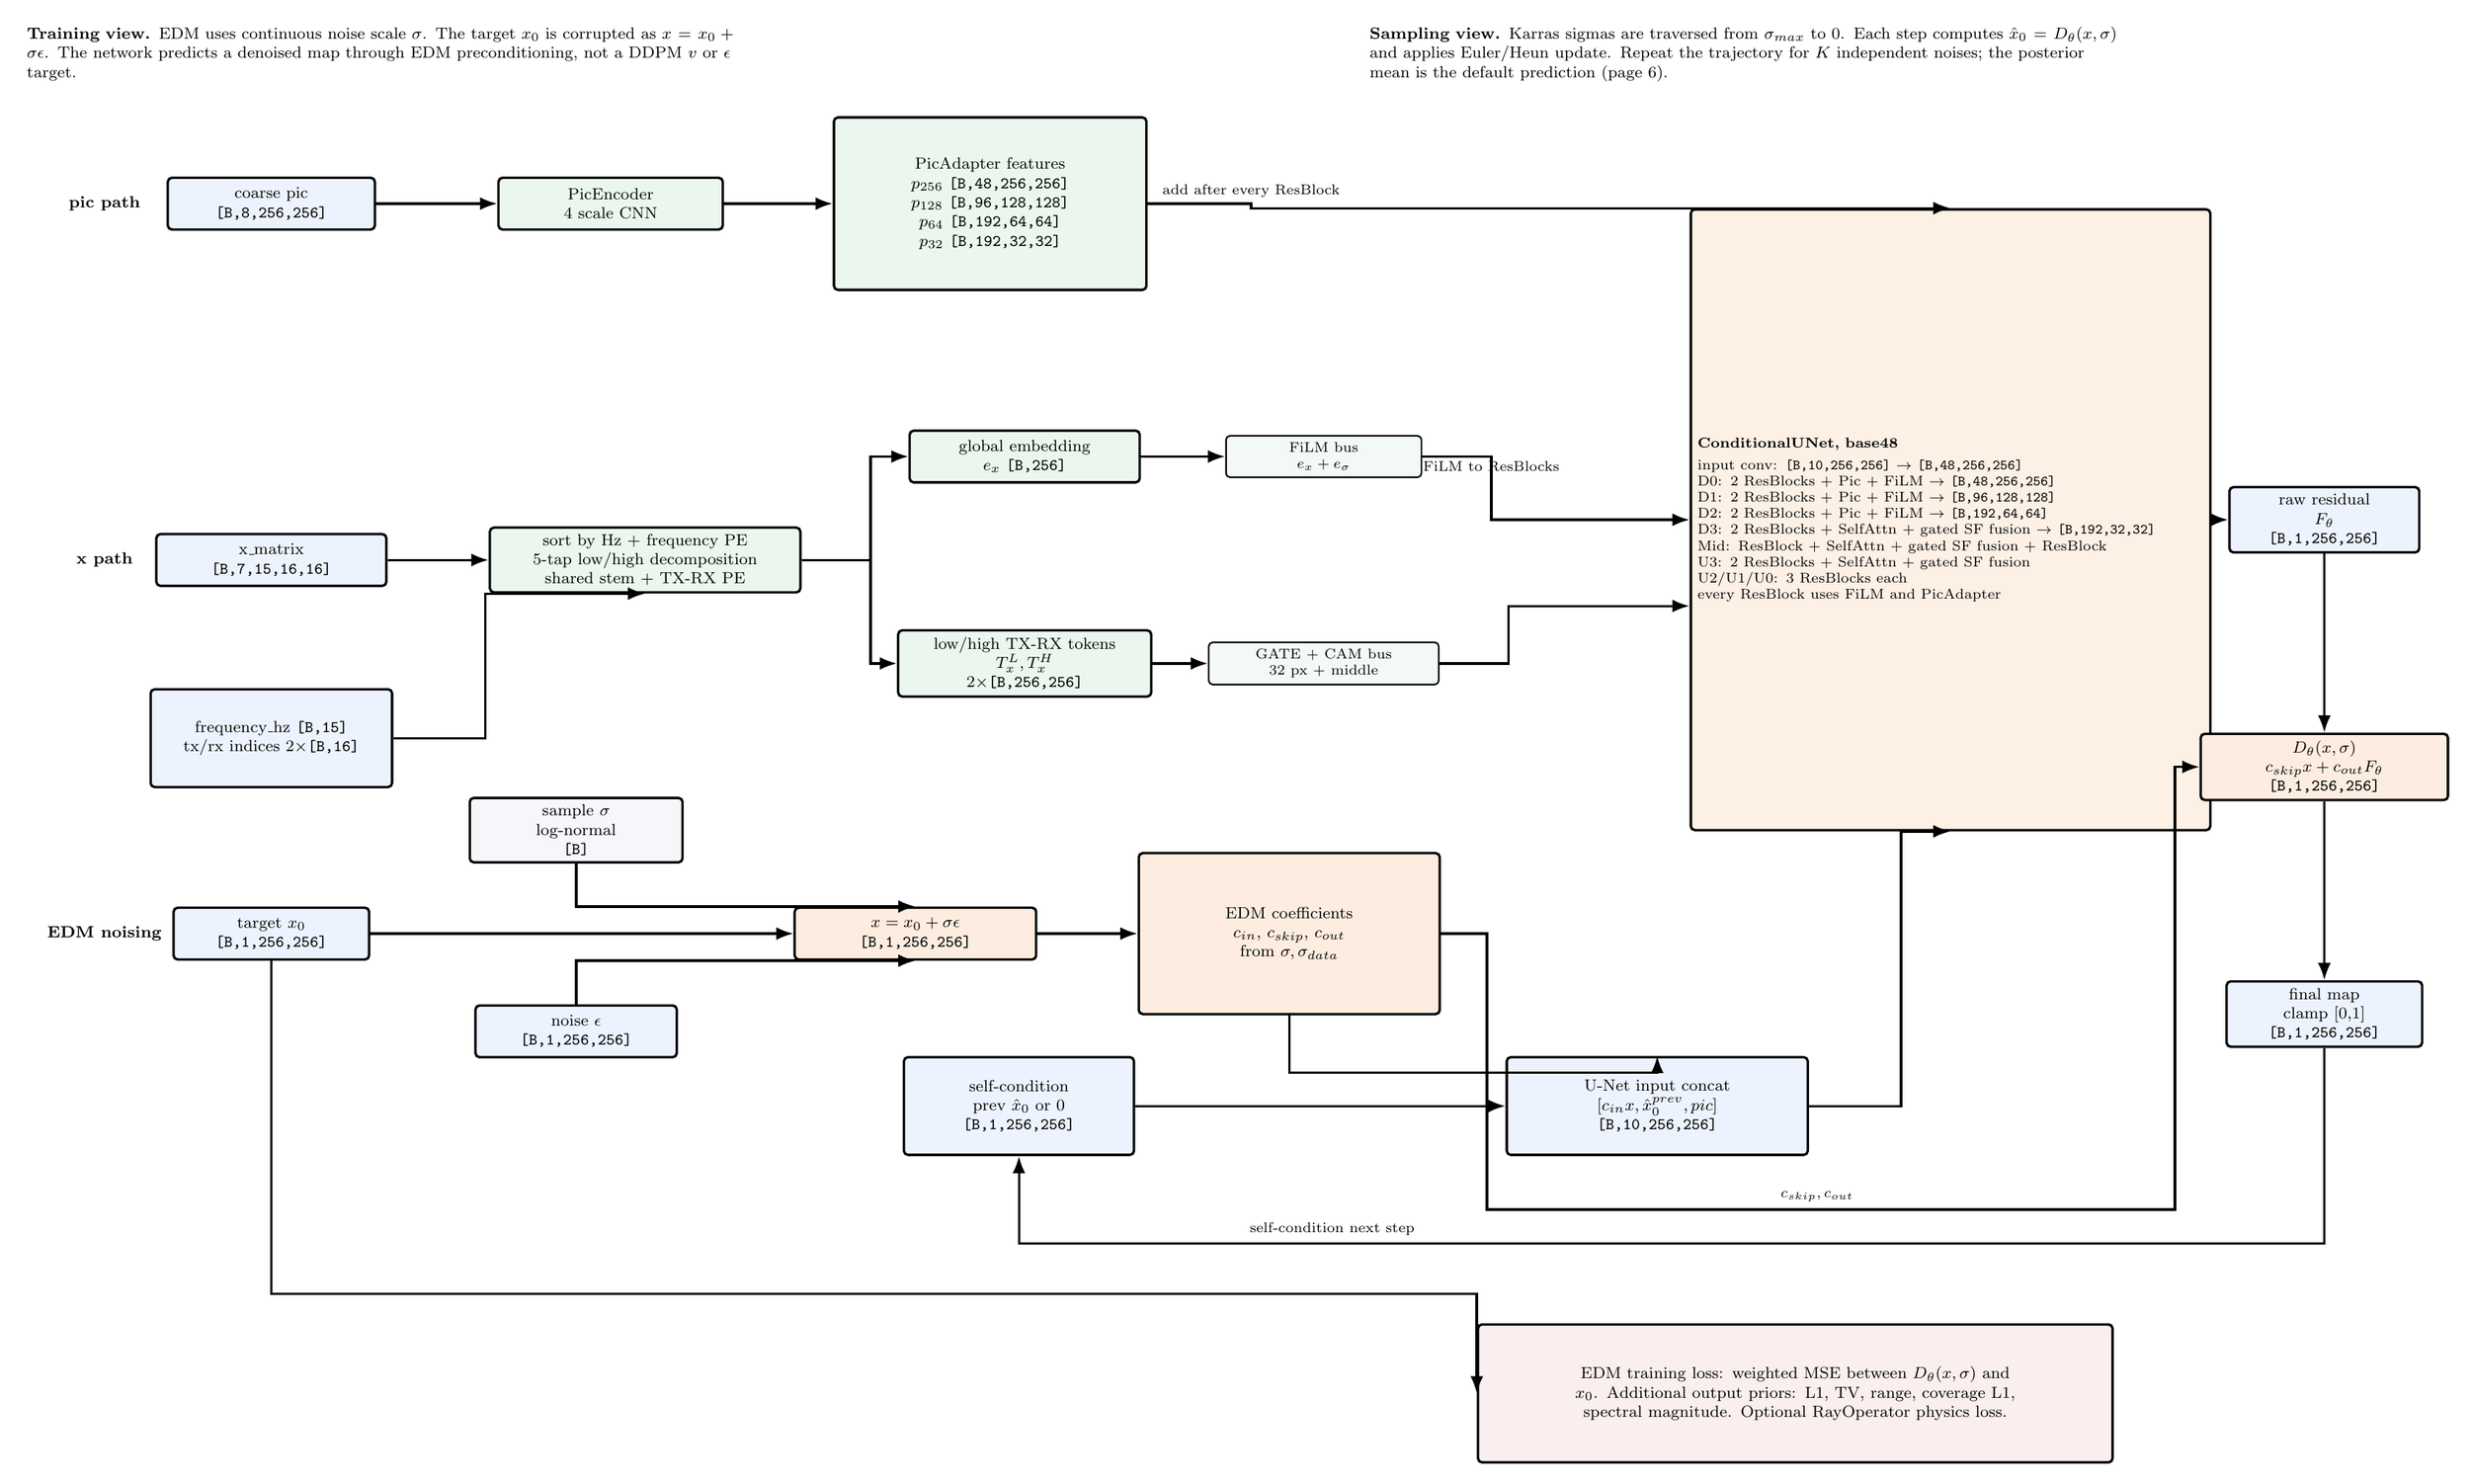
\begin{tikzpicture}[x=1mm,y=1mm]
  \node[note, text width=125mm] at (65,57) {
    \textbf{Training view.} EDM uses continuous noise scale $\sigma$.
    The target $x_0$ is corrupted as $x=x_0+\sigma\epsilon$.
    The network predicts a denoised map through EDM preconditioning, not a DDPM $v$ or $\epsilon$ target.
  };
  \node[note, text width=132mm] at (302,57) {
    \textbf{Sampling view.} Karras sigmas are traversed from $\sigma_{max}$ to 0.
    Each step computes $\hat{x}_0=D_\theta(x,\sigma)$ and applies Euler/Heun update.
    Repeat the trajectory for $K$ independent noises; the posterior mean is the default prediction (page 6).
  };

  \node[note] at (16,31) {\textbf{pic path}};
  \node[tensor, minimum width=36mm] (pic) at (45,31) {coarse pic\\\shape{B,8,256,256}};
  \node[cond, minimum width=39mm] (picenc) at (104,31) {PicEncoder\\4 scale CNN};
  \node[cond, text width=52mm, minimum height=30mm] (pfeat) at (170,31) {
    PicAdapter features\\
    $p_{256}$ \shape{B,48,256,256}\\
    $p_{128}$ \shape{B,96,128,128}\\
    $p_{64}$ \shape{B,192,64,64}\\
    $p_{32}$ \shape{B,192,32,32}
  };

  \node[note] at (16,-31) {\textbf{x path}};
  \node[tensor, minimum width=40mm] (xmat) at (45,-31) {x\_matrix\\\shape{B,7,15,16,16}};
  \node[tensor, minimum width=42mm, minimum height=17mm] (xcoord) at (45,-62) {frequency\_hz \shape{B,15}\\tx/rx indices $2\times$\shape{B,16}};
  \node[cond, minimum width=54mm] (xenc) at (110,-31) {sort by Hz + frequency PE\\5-tap low/high decomposition\\shared stem + TX-RX PE};
  \node[cond, minimum width=40mm] (emb) at (176,-13) {global embedding\\$e_x$ \shape{B,256}};
  \node[cond, minimum width=44mm] (tok) at (176,-49) {low/high TX-RX tokens\\$T_x^L,T_x^H$\\$2\times$\shape{B,256,256}};
  \node[bus, minimum width=34mm] (film) at (228,-13) {FiLM bus\\$e_x+e_\sigma$};
  \node[bus, minimum width=40mm] (cross) at (228,-49) {GATE + CAM bus\\32 px + middle};

  \node[note] at (16,-96) {\textbf{EDM noising}};
  \node[tensor, minimum width=34mm] (x0) at (45,-96) {target $x_0$\\\shape{B,1,256,256}};
  \node[op, minimum width=37mm] (sigma) at (98,-78) {sample $\sigma$\\log-normal\\\shape{B}};
  \node[tensor, minimum width=35mm] (noise) at (98,-113) {noise $\epsilon$\\\shape{B,1,256,256}};
  \node[edm, minimum width=42mm] (addnoise) at (157,-96) {$x=x_0+\sigma\epsilon$\\\shape{B,1,256,256}};

  \node[edm, text width=50mm, minimum height=28mm] (precond) at (222,-96) {
    EDM coefficients\\
    $c_{in}$, $c_{skip}$, $c_{out}$\\
    from $\sigma,\sigma_{data}$
  };
  \node[tensor, text width=50mm, minimum height=17mm] (modelin) at (286,-126) {U-Net input concat\\$[c_{in}x,\hat{x}_0^{prev},pic]$\\\shape{B,10,256,256}};
  \node[tensor, minimum width=40mm, minimum height=17mm] (selfc) at (175,-126) {self-condition\\prev $\hat{x}_0$ or 0\\\shape{B,1,256,256}};

  \node[unet, text width=88mm, minimum height=108mm] (unetbox) at (337,-24) {
    \textbf{ConditionalUNet, base48}\\[1mm]
    input conv: \shape{B,10,256,256} $\rightarrow$ \shape{B,48,256,256}\\
    D0: 2 ResBlocks + Pic + FiLM $\rightarrow$ \shape{B,48,256,256}\\
    D1: 2 ResBlocks + Pic + FiLM $\rightarrow$ \shape{B,96,128,128}\\
    D2: 2 ResBlocks + Pic + FiLM $\rightarrow$ \shape{B,192,64,64}\\
    D3: 2 ResBlocks + SelfAttn + gated SF fusion $\rightarrow$ \shape{B,192,32,32}\\
    Mid: ResBlock + SelfAttn + gated SF fusion + ResBlock\\
    U3: 2 ResBlocks + SelfAttn + gated SF fusion\\
    U2/U1/U0: 3 ResBlocks each\\
    every ResBlock uses FiLM and PicAdapter
  };

  \node[tensor, minimum width=33mm] (raw) at (402,-24) {raw residual\\$F_\theta$\\\shape{B,1,256,256}};
  \node[edm, minimum width=43mm] (denoise) at (402,-67) {$D_\theta(x,\sigma)$\\$c_{skip}x+c_{out}F_\theta$\\\shape{B,1,256,256}};
  \node[tensor, minimum width=34mm] (out) at (402,-110) {final map\\clamp [0,1]\\\shape{B,1,256,256}};
  \node[loss, text width=108mm, minimum height=24mm] (losses) at (310,-176) {
    EDM training loss: weighted MSE between $D_\theta(x,\sigma)$ and $x_0$.
    Additional output priors: L1, TV, range, coverage L1, spectral magnitude. Optional RayOperator physics loss.
  };

  \draw[arrow] (pic) -- (picenc);
  \draw[arrow] (picenc) -- (pfeat);
  \draw[arrow] (pfeat.east) -- ++(18,0) |- node[pos=0.17,above,font=\scriptsize]{add after every ResBlock} (unetbox.north);

  \draw[arrow] (xmat) -- (xenc);
  \draw[arrow] (xcoord.east) -- ++(16,0) |- (xenc.south);
  \draw[arrow] (xenc.east) -- ++(12,0) |- (emb.west);
  \draw[arrow] (xenc.east) -- ++(12,0) |- (tok.west);
  \draw[arrow] (emb) -- (film);
  \draw[arrow] (tok) -- (cross);
  \draw[arrow] (film.east) -- ++(12,0) |- node[pos=0.18,above,font=\scriptsize]{FiLM to ResBlocks} (unetbox.west);
  \draw[arrow] (cross.east) -- ++(12,0) |- ($(unetbox.west)+(0,-15)$);

  \draw[arrow] (x0) -- (addnoise);
  \draw[arrow] (sigma.south) |- (addnoise.north);
  \draw[arrow] (noise.north) |- (addnoise.south);
  \draw[arrow] (addnoise) -- (precond);
  \draw[arrow] (precond.south) -- ++(0,-10) -| (modelin.north);
  \draw[arrow] (selfc.east) -- (modelin.west);
  \draw[arrow] (modelin.east) -- ++(16,0) |- (unetbox.south);

  \draw[arrow] (unetbox.east) -- (raw);
  \draw[arrow] (raw) -- (denoise);
  \draw[arrow] (precond.east) -- ++(8,0) -- ++(0,-48)
    -- node[pos=0.48,above,font=\scriptsize]{$c_{skip},c_{out}$} (376,-144)
    -- (376,-67) -- (denoise.west);
  \draw[arrow] (denoise) -- (out);
  \draw[arrow] (x0.south) -- ++(0,-58) -| (losses.west);
  \draw[arrow] (out.south) -- ++(0,-34) -| node[pos=0.38,above,font=\scriptsize]{self-condition next step} (selfc.south);
\end{tikzpicture}

\newpage

\begin{center}
{\Large EDM Preconditioning and Tensor Shapes}\\[1mm]
{\small EDM preconditioning is combined with dynamic physical-frequency decomposition and gated spatial-frequency fusion.}
\end{center}

\small
\begin{tabular}{>{\raggedright\arraybackslash}p{37mm} >{\raggedright\arraybackslash}p{77mm} >{\raggedright\arraybackslash}p{50mm} >{\raggedright\arraybackslash}p{232mm}}
\toprule
Stage & EDM formula / operation & Shape & Purpose \\
\midrule
Clean target & $x_0$ & \shape{B,1,256,256} & Ground-truth defect-depth label. \\
Noise scale sampling & $\log\sigma \sim \mathcal{N}(p_{mean},p_{std}^2)$, clamp to $[\sigma_{min},\sigma_{max}]$ & \shape{B} & Continuous EDM training noise level. Base48 config uses $\sigma_{data}=0.5$, $\sigma_{min}=0.002$, $\sigma_{max}=80$, $p_{mean}=-1.2$, $p_{std}=1.2$. \\
Noisy image & $x=x_0+\sigma\epsilon$ & \shape{B,1,256,256} & No forward Markov chain or beta schedule is used. \\
Coefficients & $c_{in}=1/\sqrt{\sigma^2+\sigma_{data}^2}$; $c_{skip}=\sigma_{data}^2/(\sigma^2+\sigma_{data}^2)$; $c_{out}=\sigma\sigma_{data}/\sqrt{\sigma^2+\sigma_{data}^2}$ & broadcast to image dims & Stabilizes network input/output scale across noise levels. \\
Network input & $\mathrm{concat}(c_{in}x,\hat{x}_0^{prev},pic)$ & \shape{B,10,256,256} & Same channel count as DDPM version, but the first channel is preconditioned noisy input. \\
Noise embedding & $e_\sigma=\mathrm{TimeEmbedding}(\log\sigma/4)$ & \shape{B,256} & Reuses the U-Net time-embedding module with EDM's continuous log-sigma coordinate. \\
Condition vector & $c=e_x+e_\sigma$ & \shape{B,256} & FiLM condition for every ResBlock. \\
Physical-frequency tokens & sort by real Hz; inject frequency PE before aggregation; dynamic 5-tap LPF; shared stem; add TX-RX physical PE & $T_x^L,T_x^H$: $2\times$\shape{B,256,256} & Each token represents one TX-RX cell; all 15 real frequencies are encoded before tokenization. \\
Raw U-Net output & $F_\theta(c_{in}x,\hat{x}_0^{prev},pic,e_x,T_x^L,T_x^H,\sigma)$ & \shape{B,1,256,256} & Network residual after gated spatial-frequency fusion. \\
Denoised output & $D_\theta(x,\sigma)=c_{skip}x+c_{out}F_\theta$ & \shape{B,1,256,256} & Direct clean-map prediction. \\
Training loss & $\mathrm{E}_{x_0,\epsilon,\sigma}\left[w(\sigma)\lVert D_\theta(x,\sigma)-x_0\rVert_2^2\right]$; $w=(\sigma^2+\sigma_{data}^2)/(\sigma\sigma_{data})^2$ & scalar & Replaces DDPM's MSE on $v$ or $\epsilon$. \\
\bottomrule
\end{tabular}

\vspace{5mm}

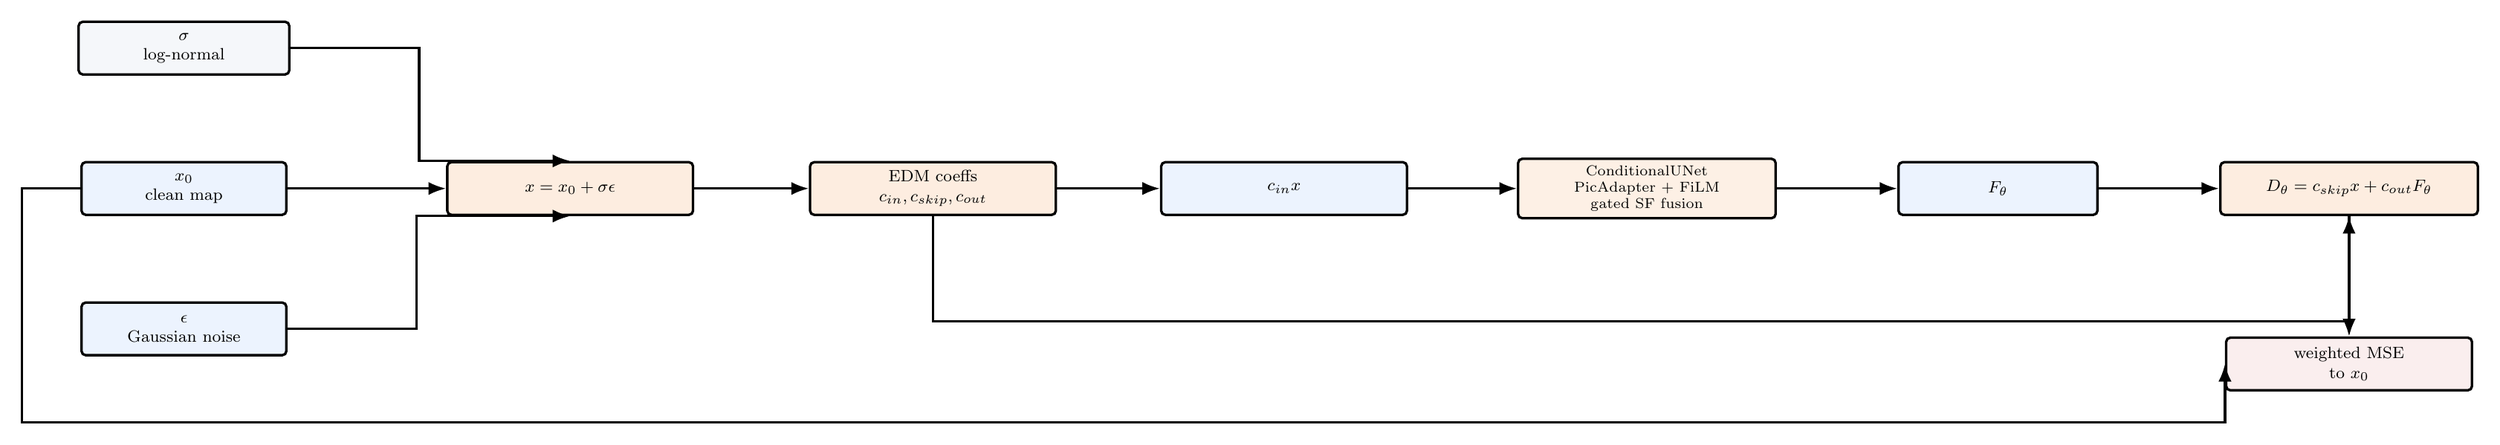
\begin{tikzpicture}[x=1mm,y=1mm]
  \node[tensor, minimum width=35mm] (x0) at (22,0) {$x_0$\\clean map};
  \node[tensor, minimum width=35mm] (eps) at (22,-24) {$\epsilon$\\Gaussian noise};
  \node[op, minimum width=36mm] (sig) at (22,24) {$\sigma$\\log-normal};
  \node[edm, minimum width=42mm] (noisy) at (88,0) {$x=x_0+\sigma\epsilon$};
  \node[edm, minimum width=42mm] (coef) at (150,0) {EDM coeffs\\$c_{in},c_{skip},c_{out}$};
  \node[tensor, minimum width=42mm] (cin) at (210,0) {$c_{in}x$};
  \node[unet, align=center, minimum width=44mm] (unet) at (272,0) {ConditionalUNet\\PicAdapter + FiLM\\gated SF fusion};
  \node[tensor, minimum width=34mm] (raw) at (332,0) {$F_\theta$};
  \node[edm, minimum width=44mm] (dout) at (392,0) {$D_\theta=c_{skip}x+c_{out}F_\theta$};
  \node[loss, minimum width=42mm] (loss) at (392,-30) {weighted MSE\\to $x_0$};

  \draw[arrow] (x0) -- (noisy);
  \draw[arrow] (eps.east) -- ++(22,0) |- (noisy.south);
  \draw[arrow] (sig.east) -- ++(22,0) |- (noisy.north);
  \draw[arrow] (noisy) -- (coef);
  \draw[arrow] (coef) -- (cin);
  \draw[arrow] (cin) -- (unet);
  \draw[arrow] (unet) -- (raw);
  \draw[arrow] (raw) -- (dout);
  \draw[arrow] (coef.south) -- ++(0,-18) -| (dout.south);
  \draw[arrow] (x0.west) -- ++(-10,0) -- ++(0,-40) -| (loss.west);
  \draw[arrow] (dout) -- (loss);
\end{tikzpicture}

\newpage

\begin{center}
{\Large Physical Frequency and TX-RX Position Encoding}\\[1mm]
{\small Real Hz is encoded before frequency aggregation; cylindrical TX-RX geometry is added after token projection.}
\end{center}

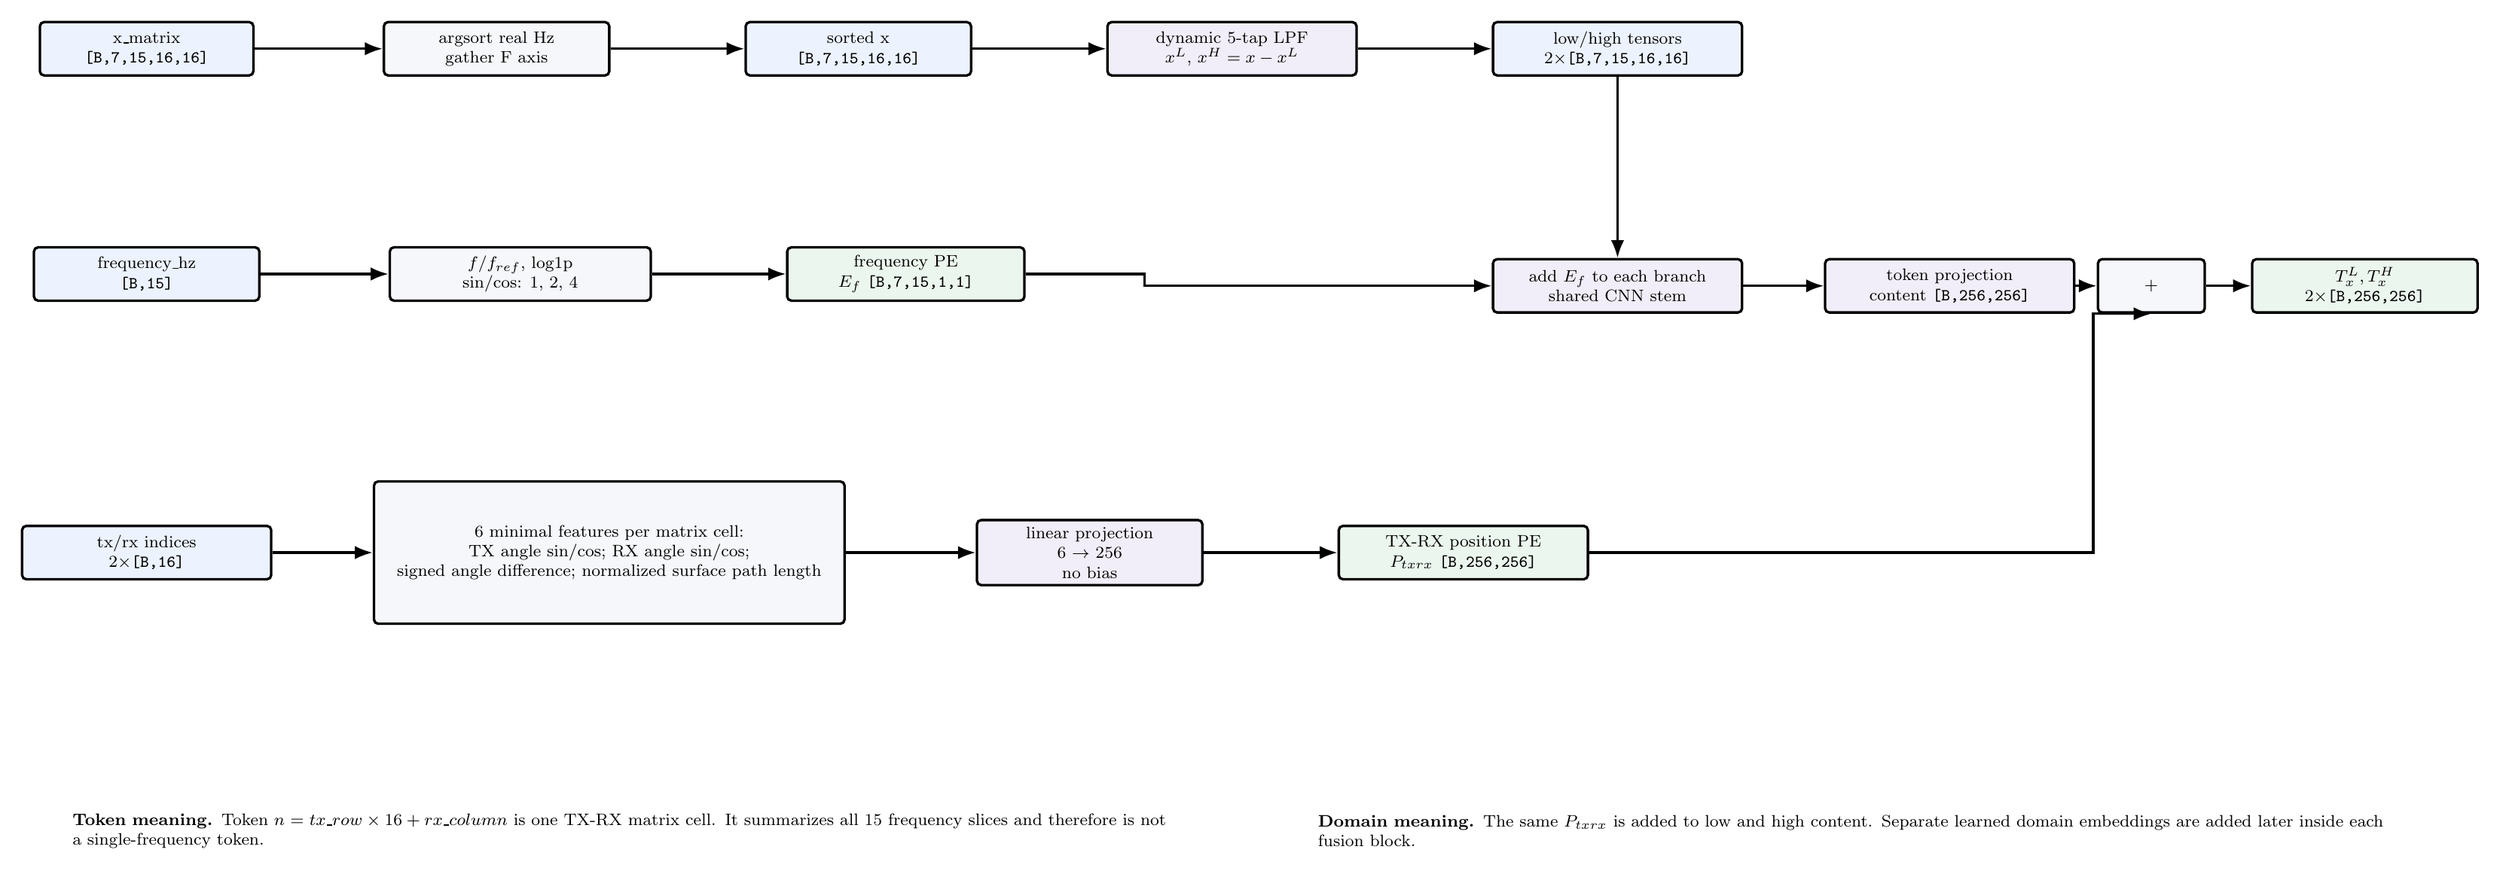
\begin{tikzpicture}[x=1mm,y=1mm]
  \node[tensor, minimum width=36mm] (px) at (25,50) {x\_matrix\\\shape{B,7,15,16,16}};
  \node[op, minimum width=38mm] (sort) at (84,50) {argsort real Hz\\gather F axis};
  \node[tensor, minimum width=38mm] (sorted) at (145,50) {sorted x\\\shape{B,7,15,16,16}};
  \node[block, minimum width=42mm] (fdgm) at (208,50) {dynamic 5-tap LPF\\$x^L$, $x^H=x-x^L$};
  \node[tensor, minimum width=42mm] (bands) at (273,50) {low/high tensors\\$2\times$\shape{B,7,15,16,16}};

  \node[tensor, minimum width=38mm] (freq) at (25,12) {frequency\_hz\\\shape{B,15}};
  \node[op, minimum width=44mm] (fourier) at (88,12) {$f/f_{ref}$, log1p\\sin/cos: 1, 2, 4};
  \node[cond, minimum width=40mm] (fpe) at (153,12) {frequency PE\\$E_f$ \shape{B,7,15,1,1}};
  \node[block, minimum width=42mm] (stem) at (273,10) {add $E_f$ to each branch\\shared CNN stem};
  \node[block, minimum width=42mm] (content) at (329,10) {token projection\\content \shape{B,256,256}};
  \node[op, minimum width=18mm] (add) at (363,10) {$+$};
  \node[cond, minimum width=38mm] (ptokens) at (399,10) {$T_x^L,T_x^H$\\$2\times$\shape{B,256,256}};

  \node[tensor, minimum width=42mm] (ids) at (25,-35) {tx/rx indices\\$2\times$\shape{B,16}};
  \node[op, text width=77mm, minimum height=24mm] (geo) at (103,-35) {6 minimal features per matrix cell:\\TX angle sin/cos; RX angle sin/cos;\\signed angle difference; normalized surface path length};
  \node[block, minimum width=38mm] (posproj) at (184,-35) {linear projection\\6 $\rightarrow$ 256\\no bias};
  \node[cond, minimum width=42mm] (ppe) at (247,-35) {TX-RX position PE\\$P_{txrx}$ \shape{B,256,256}};

  \draw[arrow] (px) -- (sort);
  \draw[arrow] (sort) -- (sorted);
  \draw[arrow] (sorted) -- (fdgm);
  \draw[arrow] (fdgm) -- (bands);
  \draw[arrow] (bands.south) -- (stem.north);
  \draw[arrow] (freq) -- (fourier);
  \draw[arrow] (fourier) -- (fpe);
  \draw[arrow] (fpe.east) -- ++(20,0) |- (stem.west);
  \draw[arrow] (stem) -- (content);
  \draw[arrow] (content) -- (add);
  \draw[arrow] (add) -- (ptokens);
  \draw[arrow] (ids) -- (geo);
  \draw[arrow] (geo) -- (posproj);
  \draw[arrow] (posproj) -- (ppe);
  \draw[arrow] (ppe.east) -- ++(85,0) |- (add.south);

  \node[note, text width=185mm] at (105,-82) {
    \textbf{Token meaning.} Token $n=tx\_row\times16+rx\_column$ is one TX-RX matrix cell.
    It summarizes all 15 frequency slices and therefore is not a single-frequency token.
  };
  \node[note, text width=185mm] at (315,-82) {
    \textbf{Domain meaning.} The same $P_{txrx}$ is added to low and high content.
    Separate learned domain embeddings are added later inside each fusion block.
  };
\end{tikzpicture}

\newpage

\begin{center}
{\Large Shared Conditional Backbone}\\[1mm]
{\small PicEncoder/PicAdapter and U-Net scales remain; the x path produces physically located low/high tokens.}
\end{center}

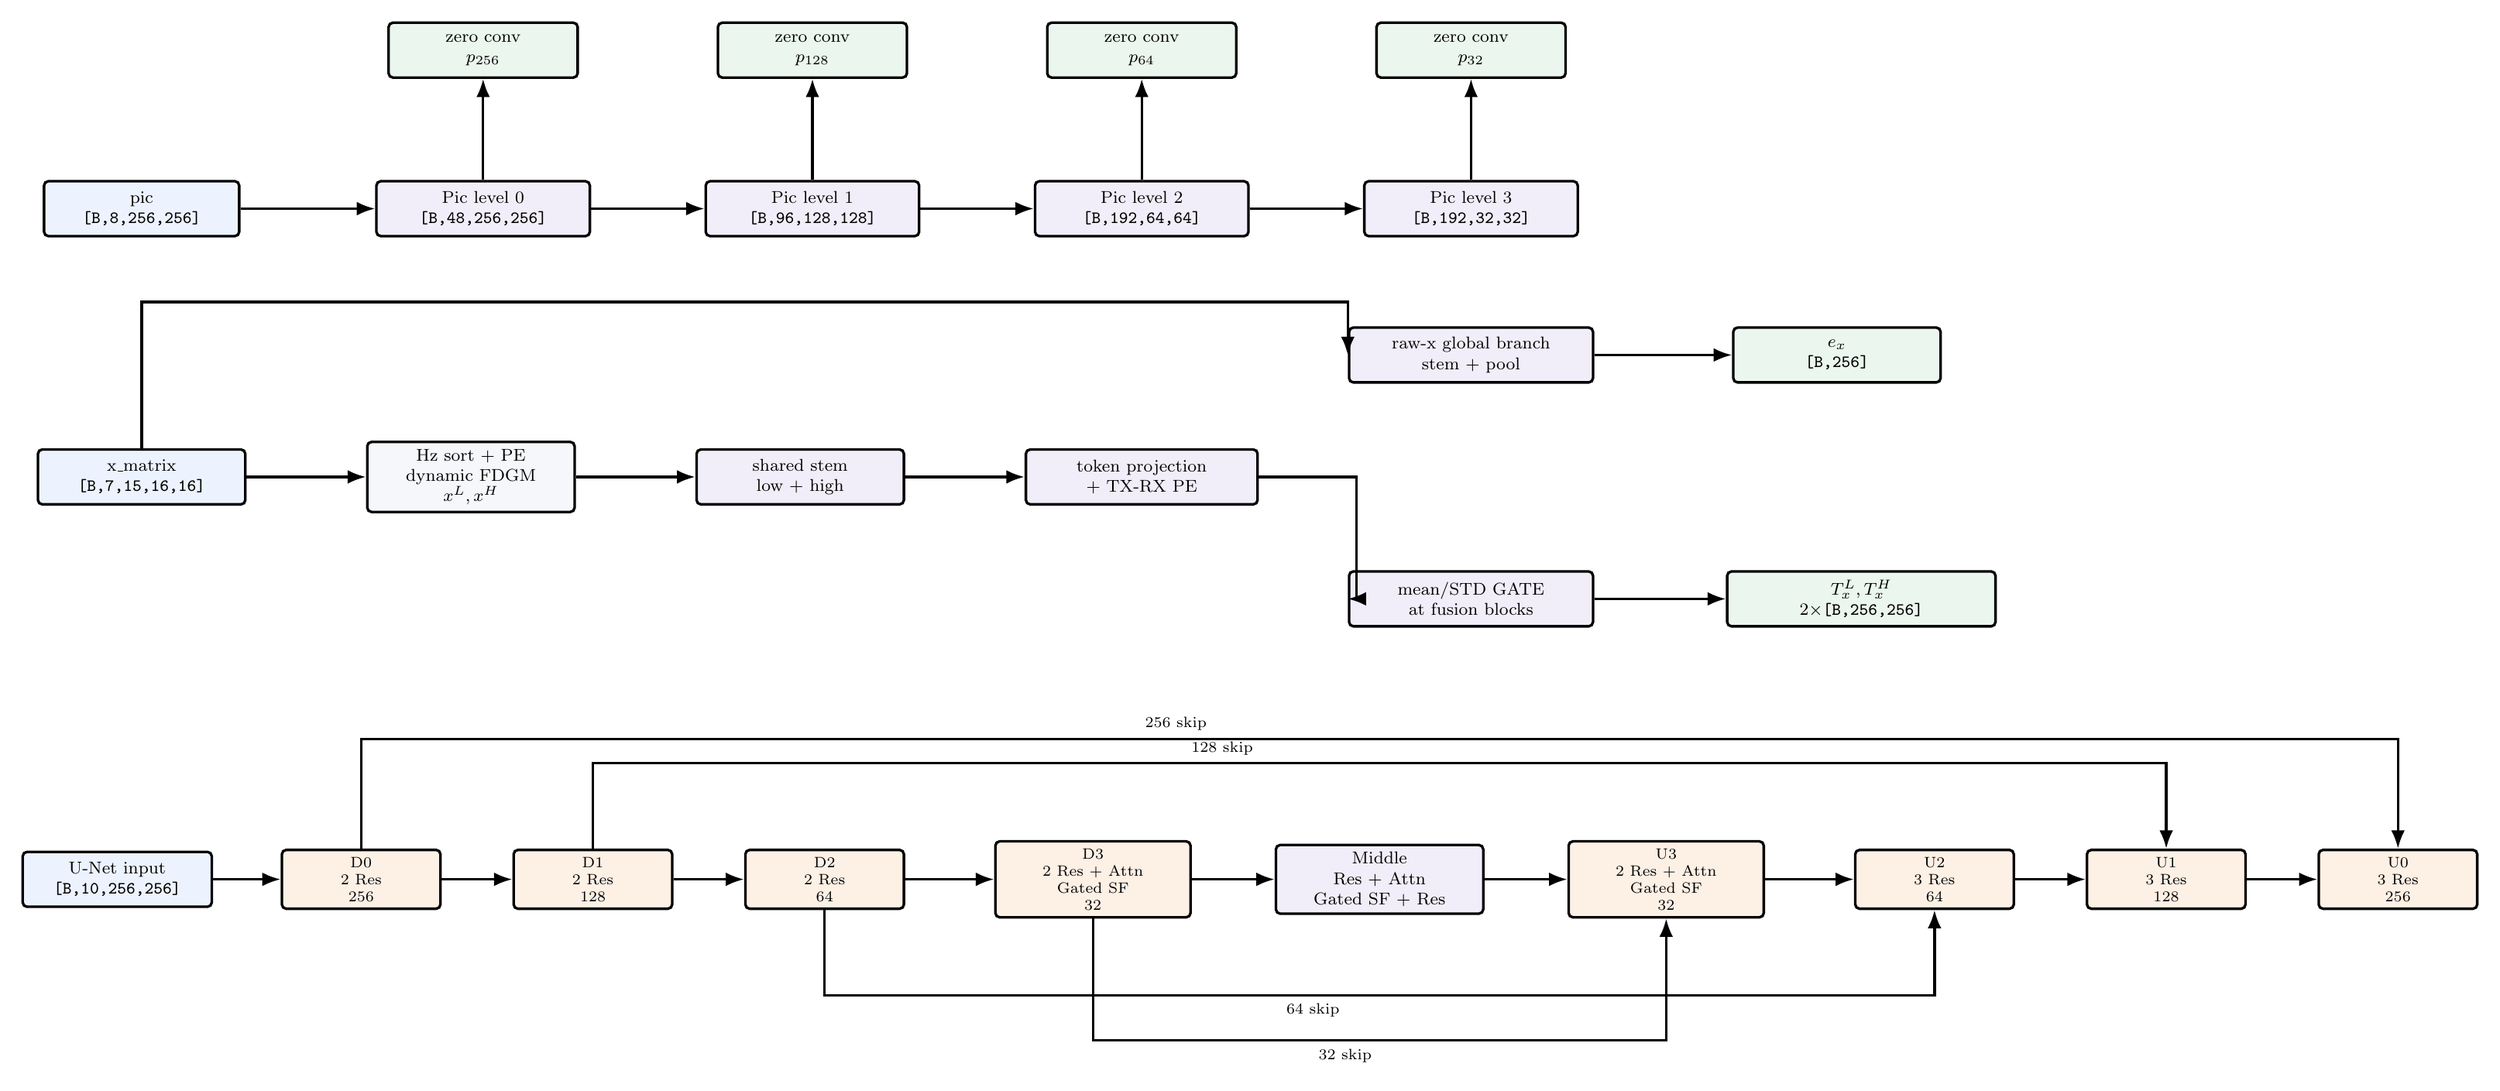
\begin{tikzpicture}[x=1mm,y=1mm]
  \node[tensor, minimum width=32mm] (picin) at (22,42) {pic\\\shape{B,8,256,256}};
  \node[block, minimum width=35mm] (p0) at (78,42) {Pic level 0\\\shape{B,48,256,256}};
  \node[block, minimum width=35mm] (p1) at (132,42) {Pic level 1\\\shape{B,96,128,128}};
  \node[block, minimum width=35mm] (p2) at (186,42) {Pic level 2\\\shape{B,192,64,64}};
  \node[block, minimum width=35mm] (p3) at (240,42) {Pic level 3\\\shape{B,192,32,32}};
  \node[cond, minimum width=31mm] (z0) at (78,68) {zero conv\\$p_{256}$};
  \node[cond, minimum width=31mm] (z1) at (132,68) {zero conv\\$p_{128}$};
  \node[cond, minimum width=31mm] (z2) at (186,68) {zero conv\\$p_{64}$};
  \node[cond, minimum width=31mm] (z3) at (240,68) {zero conv\\$p_{32}$};

  \draw[arrow] (picin) -- (p0);
  \draw[arrow] (p0) -- (p1);
  \draw[arrow] (p1) -- (p2);
  \draw[arrow] (p2) -- (p3);
  \draw[arrow] (p0) -- (z0);
  \draw[arrow] (p1) -- (z1);
  \draw[arrow] (p2) -- (z2);
  \draw[arrow] (p3) -- (z3);

  \node[tensor, minimum width=34mm] (xm) at (22,-2) {x\_matrix\\\shape{B,7,15,16,16}};
  \node[op, minimum width=34mm] (reshape) at (76,-2) {Hz sort + PE\\dynamic FDGM\\$x^L,x^H$};
  \node[block, minimum width=34mm] (stem1) at (130,-2) {shared stem\\low + high};
  \node[block, minimum width=38mm] (stem2) at (186,-2) {token projection\\+ TX-RX PE};
  \node[block, minimum width=40mm] (global) at (240,18) {raw-x global branch\\stem + pool};
  \node[cond, minimum width=34mm] (emb) at (300,18) {$e_x$\\\shape{B,256}};
  \node[block, minimum width=40mm] (tokenb) at (240,-22) {mean/STD GATE\\at fusion blocks};
  \node[cond, minimum width=44mm] (tokens) at (304,-22) {$T_x^L,T_x^H$\\$2\times$\shape{B,256,256}};

  \draw[arrow] (xm) -- (reshape);
  \draw[arrow] (reshape) -- (stem1);
  \draw[arrow] (stem1) -- (stem2);
  \draw[arrow] (xm.north) -- ++(0,24) -| (global.west);
  \draw[arrow] (global) -- (emb);
  \draw[arrow] (stem2.east) -- ++(16,0) |- (tokenb.west);
  \draw[arrow] (tokenb) -- (tokens);

  \node[tensor, minimum width=31mm] (input) at (18,-68) {U-Net input\\\shape{B,10,256,256}};
  \node[unet, align=center, minimum width=26mm] (d0) at (58,-68) {D0\\2 Res\\256};
  \node[unet, align=center, minimum width=26mm] (d1) at (96,-68) {D1\\2 Res\\128};
  \node[unet, align=center, minimum width=26mm] (d2) at (134,-68) {D2\\2 Res\\64};
  \node[unet, align=center, minimum width=32mm] (d3) at (178,-68) {D3\\2 Res + Attn\\Gated SF\\32};
  \node[block, minimum width=34mm] (mid) at (225,-68) {Middle\\Res + Attn\\Gated SF + Res};
  \node[unet, align=center, minimum width=32mm] (u3) at (272,-68) {U3\\2 Res + Attn\\Gated SF\\32};
  \node[unet, align=center, minimum width=26mm] (u2) at (316,-68) {U2\\3 Res\\64};
  \node[unet, align=center, minimum width=26mm] (u1) at (354,-68) {U1\\3 Res\\128};
  \node[unet, align=center, minimum width=26mm] (u0) at (392,-68) {U0\\3 Res\\256};

  \draw[arrow] (input) -- (d0);
  \draw[arrow] (d0) -- (d1);
  \draw[arrow] (d1) -- (d2);
  \draw[arrow] (d2) -- (d3);
  \draw[arrow] (d3) -- (mid);
  \draw[arrow] (mid) -- (u3);
  \draw[arrow] (u3) -- (u2);
  \draw[arrow] (u2) -- (u1);
  \draw[arrow] (u1) -- (u0);

  \draw[arrow] (d0.north) -- ++(0,18) -| node[pos=0.20,above,font=\scriptsize]{256 skip} (u0.north);
  \draw[arrow] (d1.north) -- ++(0,14) -| node[pos=0.20,above,font=\scriptsize]{128 skip} (u1.north);
  \draw[arrow] (d2.south) -- ++(0,-14) -| node[pos=0.22,below,font=\scriptsize]{64 skip} (u2.south);
  \draw[arrow] (d3.south) -- ++(0,-20) -| node[pos=0.22,below,font=\scriptsize]{32 skip} (u3.south);
\end{tikzpicture}

\newpage

\begin{center}
{\Large EDM Single-Trajectory Sampling and Physics Guidance}
\end{center}

\small
\begin{tabular}{>{\raggedright\arraybackslash}p{48mm} >{\raggedright\arraybackslash}p{338mm}}
\toprule
Component & EDM behavior in code \\
\midrule
Sigma schedule & \texttt{karras\_sigmas(steps)} creates a monotonically decreasing sequence from $\sigma_{max}$ to $\sigma_{min}$ and appends 0. The base48 config uses 32 sampling steps by default. \\
Initial image & Posterior draw $k$ starts from independent $z_k\sim\mathcal{N}(0,I)$ and $x_k=\sigma_{max}z_k$ with shape \shape{B,1,256,256}. \\
First denoise & Compute $\hat{x}_0=D_\theta(x,\sigma)$ using the same pic and x\_matrix conditions as training. \\
ODE derivative & $d=(x-\hat{x}_0)/\sigma$. This replaces DDPM posterior mean/variance formulas. \\
Euler/Heun update & First predicts $x_{next}=x+(\sigma_{next}-\sigma)d$, then optionally recomputes denoising at $\sigma_{next}$ and averages derivatives. \\
Self-conditioning & The current denoised output is fed as $\hat{x}_0^{prev}$ in the next denoising call. \\
Physics guidance & After a configured fraction of sampling steps, $\hat{x}_0$ can be adjusted by the gradient of frequency-aware RayOperator consistency loss before forming the ODE derivative. \\
\bottomrule
\end{tabular}

\vspace{6mm}

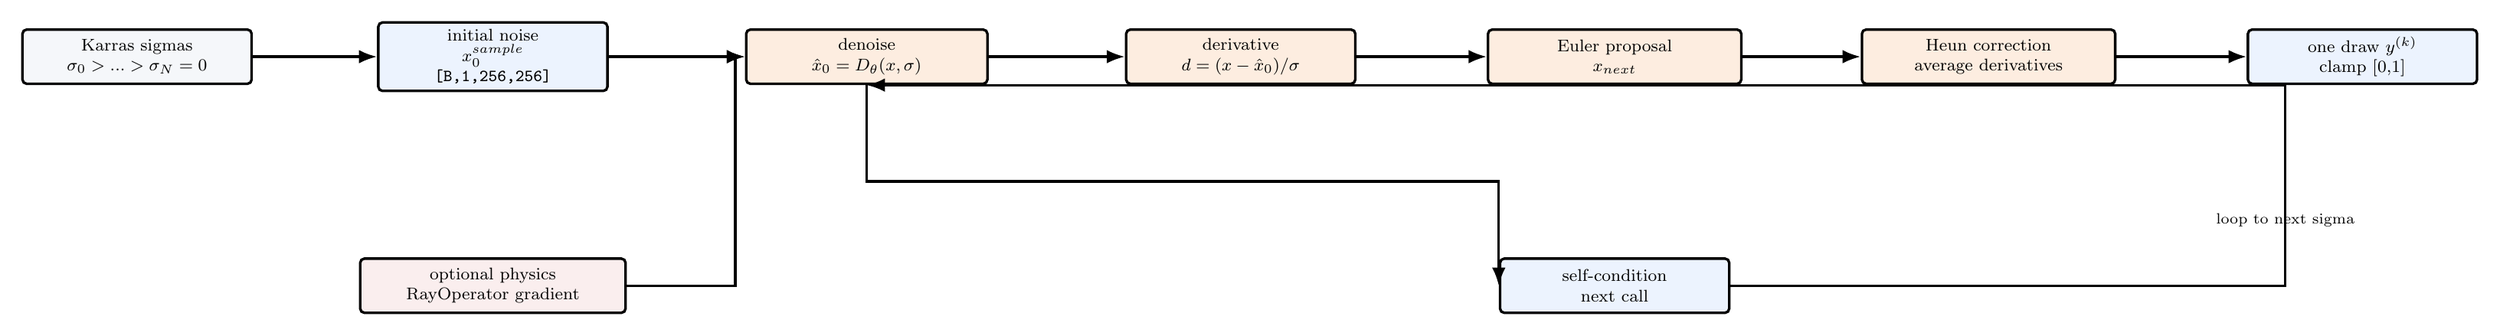
\begin{tikzpicture}[x=1mm,y=1mm]
  \node[op, minimum width=38mm] (sigmas) at (25,20) {Karras sigmas\\$\sigma_0 > ... > \sigma_N=0$};
  \node[tensor, minimum width=38mm] (init) at (84,20) {initial noise\\$x_0^{sample}$\\\shape{B,1,256,256}};
  \node[edm, minimum width=40mm] (denoise) at (146,20) {denoise\\$\hat{x}_0=D_\theta(x,\sigma)$};
  \node[loss, minimum width=44mm] (phys) at (84,-18) {optional physics\\RayOperator gradient};
  \node[edm, minimum width=38mm] (deriv) at (208,20) {derivative\\$d=(x-\hat{x}_0)/\sigma$};
  \node[edm, minimum width=42mm] (euler) at (270,20) {Euler proposal\\$x_{next}$};
  \node[edm, minimum width=42mm] (heun) at (332,20) {Heun correction\\average derivatives};
  \node[tensor, minimum width=38mm] (final) at (394,20) {one draw $y^{(k)}$\\clamp [0,1]};
  \node[tensor, minimum width=38mm] (selfc) at (270,-18) {self-condition\\next call};

  \draw[arrow] (sigmas) -- (init);
  \draw[arrow] (init) -- (denoise);
  \draw[arrow] (denoise) -- (deriv);
  \draw[arrow] (deriv) -- (euler);
  \draw[arrow] (euler) -- (heun);
  \draw[arrow] (heun) -- (final);
  \draw[arrow] (phys.east) -- ++(18,0) |- (denoise.west);
  \draw[arrow] (denoise.south) -- ++(0,-16) -| (selfc.west);
  \draw[arrow] (selfc.east) -- ++(92,0) |- node[pos=0.20,below,font=\scriptsize]{loop to next sigma} (denoise.south);
\end{tikzpicture}

\vspace{7mm}

\begin{tabular}{>{\raggedright\arraybackslash}p{58mm} >{\raggedright\arraybackslash}p{328mm}}
\toprule
Difference from diffusion & Summary \\
\midrule
Training target & Diffusion predicts $v$ by default and recovers $x_0$ from $y_t,t,v$. EDM directly trains the denoised output $D_\theta(x,\sigma)$ against $x_0$. \\
Noise variable & Diffusion uses integer timestep $t$ and beta schedule. EDM uses continuous $\sigma$ and log-normal training noise distribution. \\
Sampler & Diffusion uses DDPM/DDIM formulas. EDM uses Karras sigma schedule and ODE-style Euler/Heun updates. \\
Backbone & EDM now adds dynamic physical-frequency decomposition and gated SF fusion; PicEncoder/PicAdapter, FiLM, U-Net scales, and RayOperator remain. \\
\bottomrule
\end{tabular}

\newpage

\begin{center}
{\Large Single-Model Multi-Sample Posterior and Uncertainty Maps}\\[1mm]
{\small The condition and network weights remain fixed; only the initial EDM noise changes across posterior draws.}
\end{center}

\vspace{5mm}

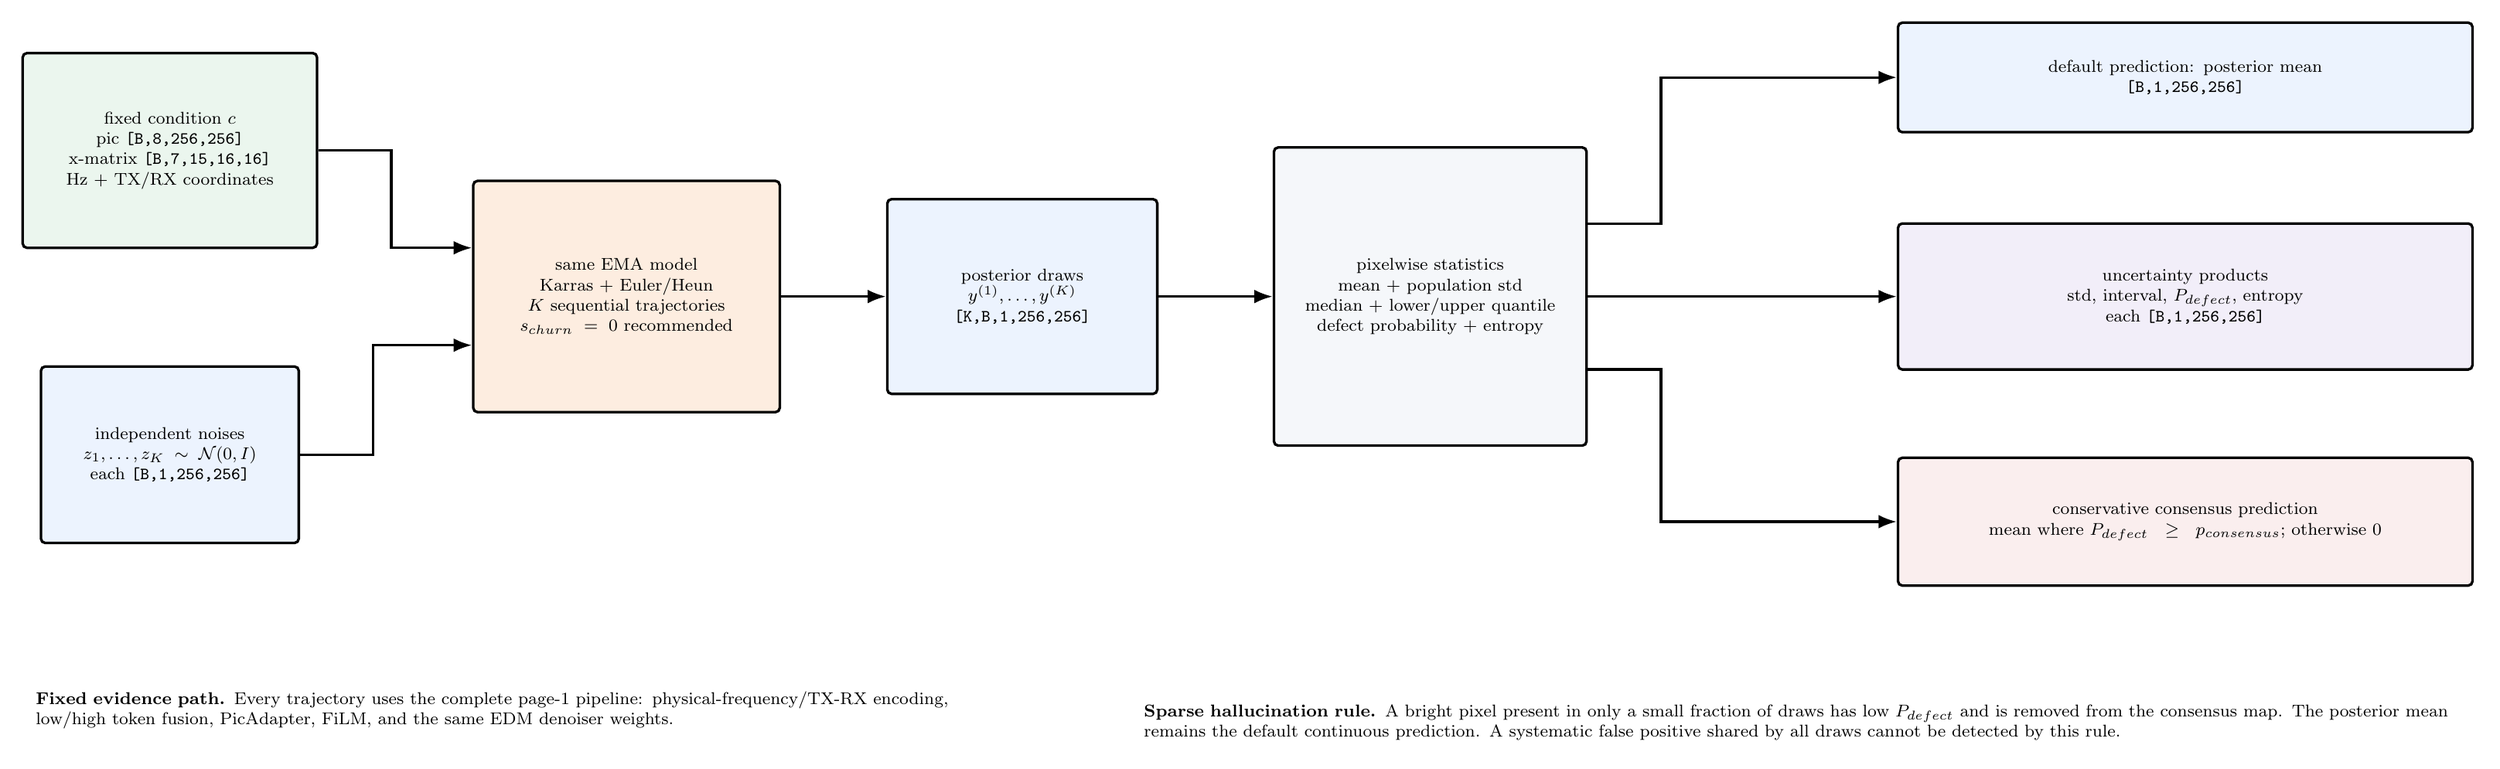
\begin{tikzpicture}[x=1mm,y=1mm]
  \node[cond, text width=46mm, minimum height=32mm] (condition) at (31,75) {
    fixed condition $c$\\
    pic \shape{B,8,256,256}\\
    x-matrix \shape{B,7,15,16,16}\\
    Hz + TX/RX coordinates
  };
  \node[tensor, text width=40mm, minimum height=29mm] (noisebank) at (31,25) {
    independent noises\\
    $z_1,\ldots,z_K\sim\mathcal{N}(0,I)$\\
    each \shape{B,1,256,256}
  };
  \node[edm, text width=48mm, minimum height=38mm] (samplerbank) at (106,51) {
    same EMA model\\
    Karras + Euler/Heun\\
    $K$ sequential trajectories\\
    $s_{churn}=0$ recommended
  };
  \node[tensor, text width=42mm, minimum height=32mm] (draws) at (171,51) {
    posterior draws\\
    $y^{(1)},\ldots,y^{(K)}$\\
    \shape{K,B,1,256,256}
  };
  \node[op, text width=49mm, minimum height=49mm] (statistics) at (238,51) {
    pixelwise statistics\\
    mean + population std\\
    median + lower/upper quantile\\
    defect probability + entropy
  };
  \node[tensor, text width=92mm, minimum height=18mm] (meanout) at (362,87) {
    default prediction: posterior mean\\
    \shape{B,1,256,256}
  };
  \node[block, text width=92mm, minimum height=24mm] (uncout) at (362,51) {
    uncertainty products\\
    std, interval, $P_{defect}$, entropy\\
    each \shape{B,1,256,256}
  };
  \node[loss, text width=92mm, minimum height=21mm] (consensusout) at (362,14) {
    conservative consensus prediction\\
    mean where $P_{defect}\geq p_{consensus}$; otherwise 0
  };

  \draw[arrow] (condition.east) -- ++(12,0) |- ($(samplerbank.west)+(0,8)$);
  \draw[arrow] (noisebank.east) -- ++(12,0) |- ($(samplerbank.west)+(0,-8)$);
  \draw[arrow] (samplerbank) -- (draws);
  \draw[arrow] (draws) -- (statistics);
  \draw[arrow] ($(statistics.east)+(0,12)$) -- ++(12,0) |- (meanout.west);
  \draw[arrow] (statistics.east) -- (uncout.west);
  \draw[arrow] ($(statistics.east)+(0,-12)$) -- ++(12,0) |- (consensusout.west);

  \node[note, text width=150mm] at (84,-17) {
    \textbf{Fixed evidence path.} Every trajectory uses the complete page-1 pipeline:
    physical-frequency/TX-RX encoding, low/high token fusion, PicAdapter, FiLM,
    and the same EDM denoiser weights.
  };
  \node[note, text width=218mm] at (300,-19) {
    \textbf{Sparse hallucination rule.} A bright pixel present in only a small fraction of draws has low
    $P_{defect}$ and is removed from the consensus map. The posterior mean remains the default continuous
    prediction. A systematic false positive shared by all draws cannot be detected by this rule.
  };
\end{tikzpicture}

\vspace{8mm}

\begin{tabular}{>{\raggedright\arraybackslash}p{66mm} >{\raggedright\arraybackslash}p{320mm}}
\toprule
Output / metric & Definition and interpretation \\
\midrule
Posterior mean & $\mu=(1/K)\sum_k y^{(k)}$. Saved as \texttt{*\_prediction.npy}; this is the default result for MAE, RMSE, SSIM, and volume error. \\
Uncertainty map & $s=\sqrt{(1/K)\sum_k(y^{(k)}-\mu)^2}$. It measures disagreement between conditional samples, not inverse path coverage and not complete model-parameter uncertainty. \\
Defect probability & $P_{defect}=(1/K)\sum_k\mathbf{1}[y^{(k)}\geq\tau_{defect}]$. Binary entropy is highest when samples disagree about whether a defect exists. \\
Calibration checks & Report empirical interval coverage, interval width, CRPS when raw draws are retained, uncertainty-error Spearman correlation, Brier score, and uncertainty versus path coverage/reliability. \\
Recommended K & Use $K=16$ for routine inspection and $K=32$ for final stability checks. $K=2$ or 4 is only a smoke-test setting. \\
\bottomrule
\end{tabular}

\end{document}
